\documentclass{acm_proc_article-sp}

\begin{document}
\title{Share*Match, An EECS341 Project}
\subtitle{Final Project Report}
\numberofauthors{3}
\author{
\alignauthor Ian Dimayuga \\
    \email{ian.dimayuga@case.edu}\\
\alignauthor Tom Dooner \\
    \email{tom.dooner@case.edu}\\
\alignauthor Brian Stack \\
    \email{brian.stack@case.edu}
}
\maketitle
\begin{abstract}
We have developed a simple web application which uses a relational database to permit users to share items that would otherwise go unutilized in their own homes.
\end{abstract}

\section{Introduction}
% From Project Proposal 1
In the world of homeownership, it is often necessary to purchase items which are not regularly used. 
Unfortunately, these items, once purchased, often lie on shelves for months unused. 
Meanwhile, neighbors or close friends may require similar items and may purchase these items themselves if they didn't think to ask those who live around them.

ShareMatch seeks to meet this need. We have built a web application that leverages the locality of users to 
enable local connection to save money. By having users log in and be able to search for local items that fit 
their criteria, users can save money on purchasing those items for one-off uses. And, if a user happens to own 
an unusual device, he or she can list the device on the site where others can find it.

To aid this process, we will build a sort of \textit{sharing karma} system that is based on trust. 
By having users trust their real-life friends, we can prioritize search requests as well as provide 
users visual feedback of a user's real-life responsibility and likelihood to return items.

\section{Application Requirements Specification}
% From Project Proposal 1
When a user navigates to the ShareMatch homepage, he or she should see a page with pictures of items on it.
This serves to give the user an indication of what types of items have recently been shared or are new items posted. 
Clicking on an image of an item should bring the user to the page for that item upon which they can opt to b
orrow that item if it's available.

At the top of the homepage, user management links will allow people to interact with the site in a personal way. 
A ``Register'' link will take a person to another page. The registration page will be a simple page with multiple 
text fields for properties of a user, such as name, e-mail address, and password. After completing the registration, the new user will be informed that they can now log in with their e-mail address and password.

The top of the homepage will also contain a link to allow users to log in. In typical UI design, after clicking this link, the user will be presented with a box for their e-mail address and password. Clicking Login will validate their e-mail address and password, and, on correct entry, redirect them to a personalized landing page.

From the user landing page, logged-in users should be able to select their location. This will probably be implemented by a zip-code selection box. Upon entering their zip code, users will be ``joining'' the location and be sent to the location page.
On this location page, various local information will be displayed. For instance, we will show some available items in the given region along with some recently borrowed items. Naturally there will also be a list of users on this page, and clicking on their names will take you to that user's profile page. Overall, a location (ZIP code) is sort of the hub that you can go to find an item if the search method isn't working.

Upon clicking on a user's name, the browsing user will be taken to the profile page for the clicked user. A user's profile page will contain such things as a list of items that they are borrowing or have recently borrowed. Also, on the user profile page, if you are logged in, you will see a button to signify that you ``Trust'' the person.

``Trust'' is our friendship mechanism. Roughly analogous to Twitter's ''follow'', ``trust'' indicates that you want to prioritize this person's items. Items from trusted loaners will show up higher when searched for.

On a user's own profile page, the same fields show up with the addition of a button which
signifies ``offer an item to loan''. Upon clicking this page, the loaning user will be taken to a page with a few fields on it regarding the item. Example fields include a Title, a short Description, some picture uploads, and some other item data. For example, one pertinent item attribute we plan to include is a desired rental time period (for instance ``I only want to loan my punching bag out for two week segments'').

Items will be categorized into tagged categories. Upon uploading an item, the uploading user can specify a list of tags which apply to that item (e.g. ``Fitness, Boxing''). Items will leverage this ontology in search pages and on user profile pages so that users can find most efficiently their desired item.

In general, users will probably find an item via our built-in search mechanism. A large box on top of most pages will invite users to input a keyword which will be matched against item names, tags, and descriptions. The most relevant items will be returned, and the items will be ranked using a combination of trustworthiness (if you trust the other user) and keyword relevance.

The search results page will be a listed display of item images. The images will be supplimented with some other information about each item. Each item image will be clickable and take the user to a page where the user can easily request to borrow that item.

On the borrowing page, the item will be displayed along with some other data about an item. For example, on Amazon (and other e-commerce sites), users may review items to provide valuable feedback. We see this paradigm as especially important for applications like this -- so that the bad items may be avoided and the better items chosen where such options exist.

Logistically, we plan to send e-mails automatically when items are requested to be borrowed. However, we also plan to implement a basic messaging system which can be used for inter-personal communication for things such as ``Oops, I broke your item.'' In this case, we
intend to implement functionality which will allow users to follow through a slightly-more-formal process to note their problem. So, users will be able to reply, forgive, or compensate to problem reports regarding their items. When possible, problem reports will appear in the normal message stream between users.

\section{Database Requirements Specification}
% From Project Proposal 1
The name is assumed to be of the standard western format of ``first last'' for the time being, although an upgrade to international standards could be made if it were necessary. Their physical address is stored because our application interacts with the real world and we need to know this for exchange of items. The email address and join date are included for obvious reasons. Finally the password hash is a necessity to allow users to log in to the site, and be authenticated as themselves.

The item table is of a similar magnitude, containing fields for value, description, date added, and maximum loan time. The first fields are fairly self explanatory, but the maximum loan time has an interesting application in that it will be used to warn users who have borrowed an item that they are heading towards the end of their allocated time. It also has a foreign key linking it to the owner of the item.

The second way that items and users are linked is through the borrowing join table. It contains the foreign keys of both users and items, with an entry indicating that the user has at
some point borrowed the item. There are starting and ending dates to show for how long the user had the item, and a foreign key for an issue.

The issue table will be used to keep track of the state of a complaint against the user who borrowed or is lending the item. An example use case for this is that if the borrower breaks the item, they will notify the lender of this, and then it can be resolved through this. It contains keys for conversations that occur between the users in order to resolve the conflict.

The conversations are a major part of our application. They are also non-trivial although we have designed a system for them that is rather simple. All conversations are ongoing and take place between two users. There is no end to a conversation, and new ones do not begin later. This allows us to have a single message table that contains the primary keys of two users, in addition to the body of the message itself and a time of creation.

The conversation will be used in two ways. Primarily as a way for the lender and borrower to decide how they will exchange their items. Also as mentioned above, they will be used in conflict resolution when an issue occurs with a borrowing event.

An important foundation of our platform is the idea of trust between users. In order to support trustworthy users and identify non-trustworthy ones, we have implemented a simple system that is roughly analogous to ``friending'' on popular social networking sites. Users can trust one another, which must be reciprocated in order to take effect. When two users trust each other, their items will show up higher in any search for an item. Conversely, a user can block another user if they find them to be not worth borrowing or lending to, and then the blockee will not show up in any search blocker, and the blocker will not show up in any search by the blockee. This relationship is not reciprocal.

This relationship will be represented by a karma table that maps users onto users and has a single value that indicates whether the relation is a block or a trust. This is a flexible solution, and will be able to grow with the application over time.

One of the other most important elements of our application is the idea of tags. Each item can be tagged with some sort of text. The relationship is many to many, and is a way of enabling users to navigate the site more easily and for administrators to see what common categories of items are. It will be implemented as a simple table with a join table between items and tags.

In addition there is a simple table that will represent media of the item. This will allow users to upload images or video of the item in question. This table will merely contain a link to a url, not the actual binary blob of data. This is because web servers are very good at serving static files and can handle this much more efficiently than piping the data out of the database.

There is a table that exists for the purpose of aggregating users from similar locations. It is based on zipcode and will be used to find users who are near to each other in order to facilitate lending. It also has a description for the location and the time that the location first joined the community.

Finally, we have a system for reviews that contain a body of text and a foreign key for the user who posted the review. The nice part about these reviews is that they can be considered helpful or not helpful by other users, thereby creating a system where only useful comments are displayed at the top. This is implemented with a join table between users and comments.

There will be a set of queries that occur far more frequently than others, and so the application should be optimized towards these.

Primarily the actions associated with finding and displaying items will be run the most. This will necessitate selecting items from the items table. The results will be paginated so that more than 20 results don't have to be loaded every time this action occurs. In addition when an item is viewed a lot of things will need to be loaded and displayed. This means that there will be a lot of queries to comments tables and images or other media. In addition the table that checks to see if something is borrowed will be hit pretty hard.

The most important integrity constraint is that when a user ceases to exist, their items must be removed along with them. When a user deletes themselves, their comments will still exist, but just from an anonymous user. Also, when a user ceases to exist, his or her messages with others must remain intact along with all of the records of loaned or borrowed items.

\section{ER Model Data Design}
% From Project Proposal 2
Our ER Model Diagram is attached at the end as Figure \ref{fig:ERDiagram}.
\begin{figure*}[p]
    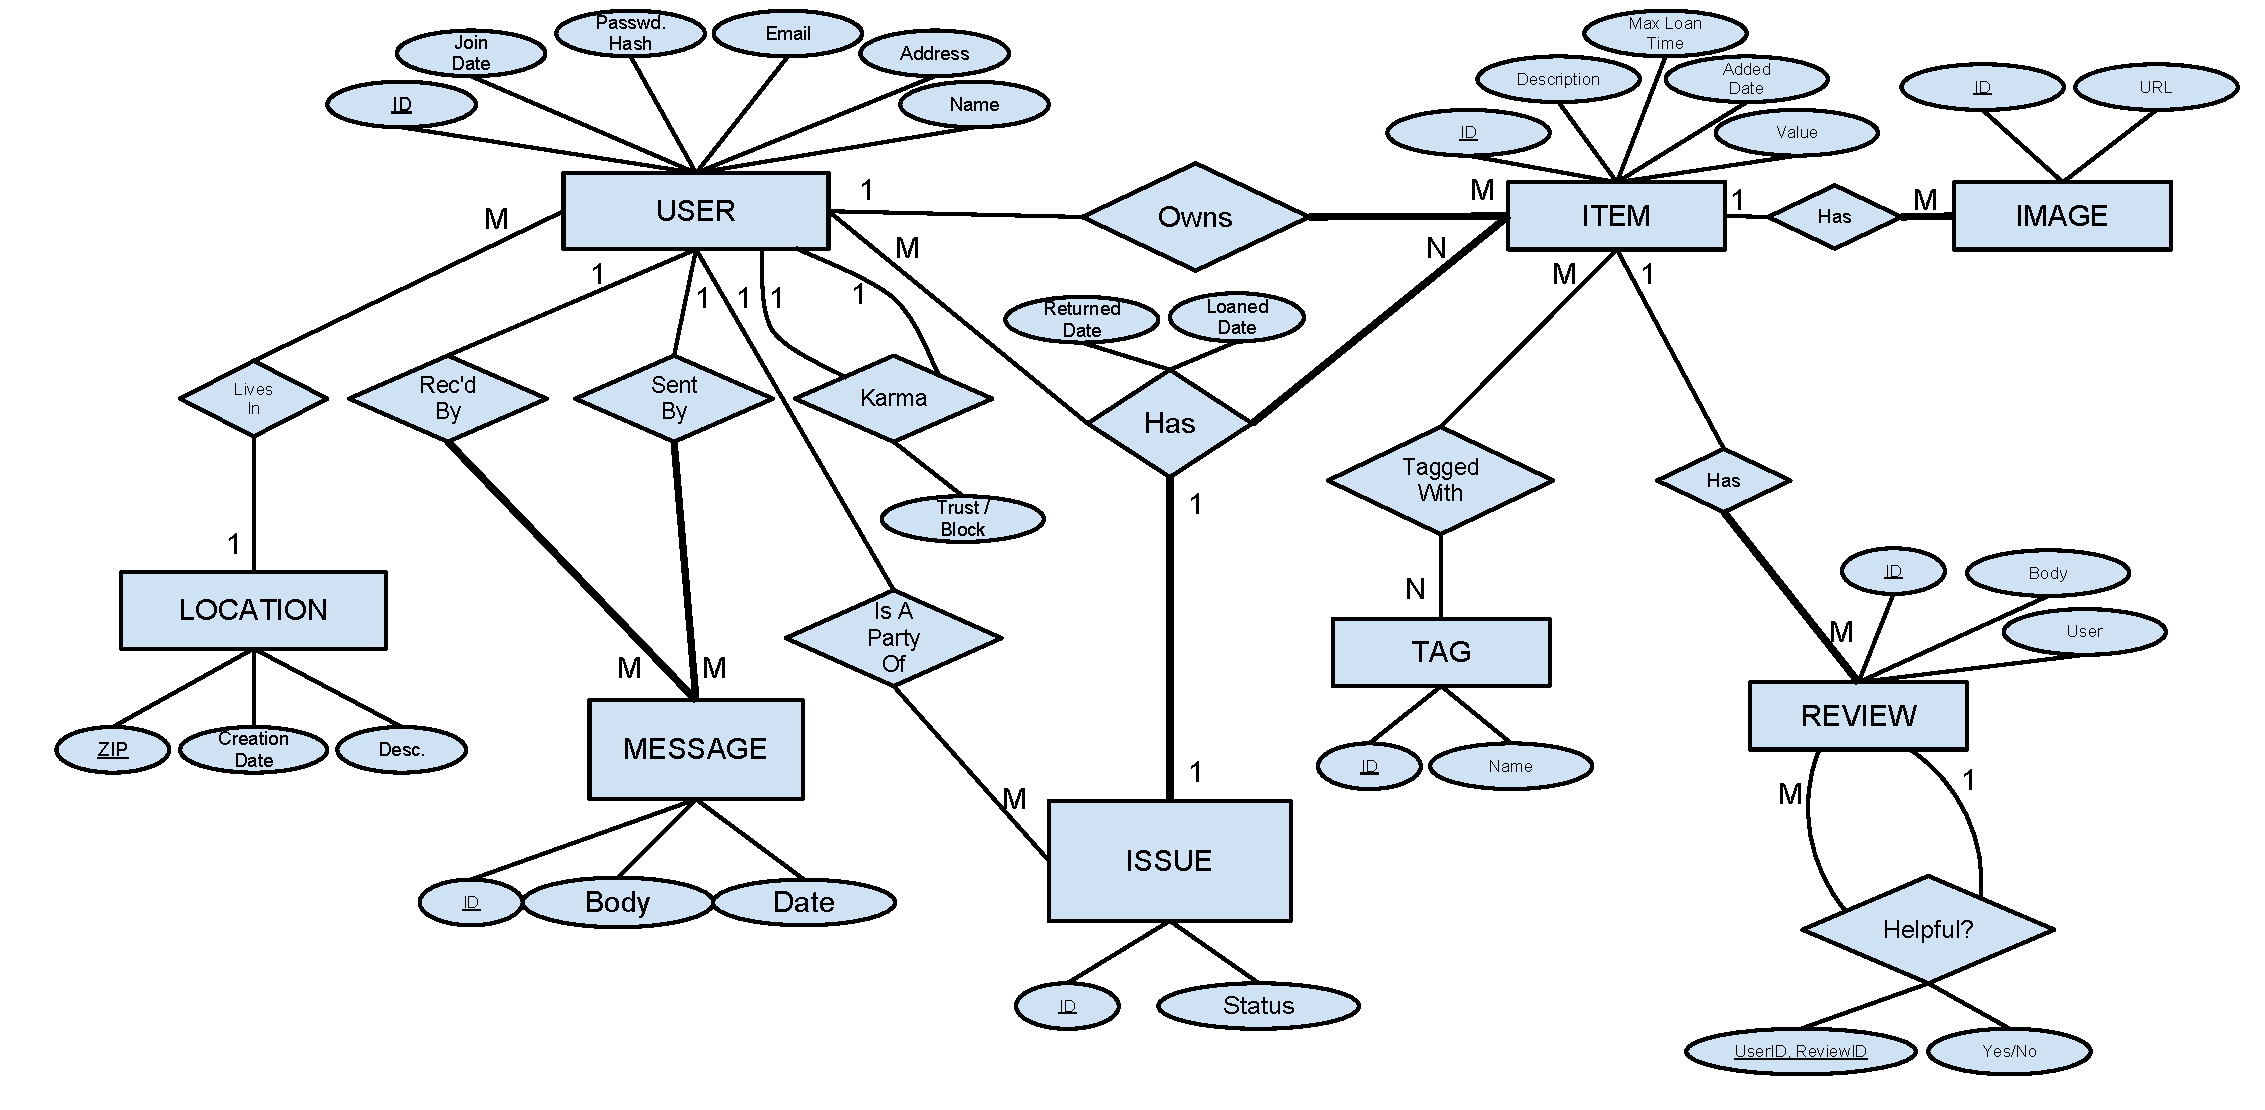
\includegraphics[width=\textwidth]{EECS341ProjectERDiagram.pdf}
    \caption{ER Diagram for Share*Match}
    \label{fig:ERDiagram}
\end{figure*}

\section{Transforming ER Model to Relational Model}
% From Project Proposal 2
Our Relational Model Diagram is attached at the end as Figure \ref{fig:RelationalDiagram}.
\begin{figure*}[p]
    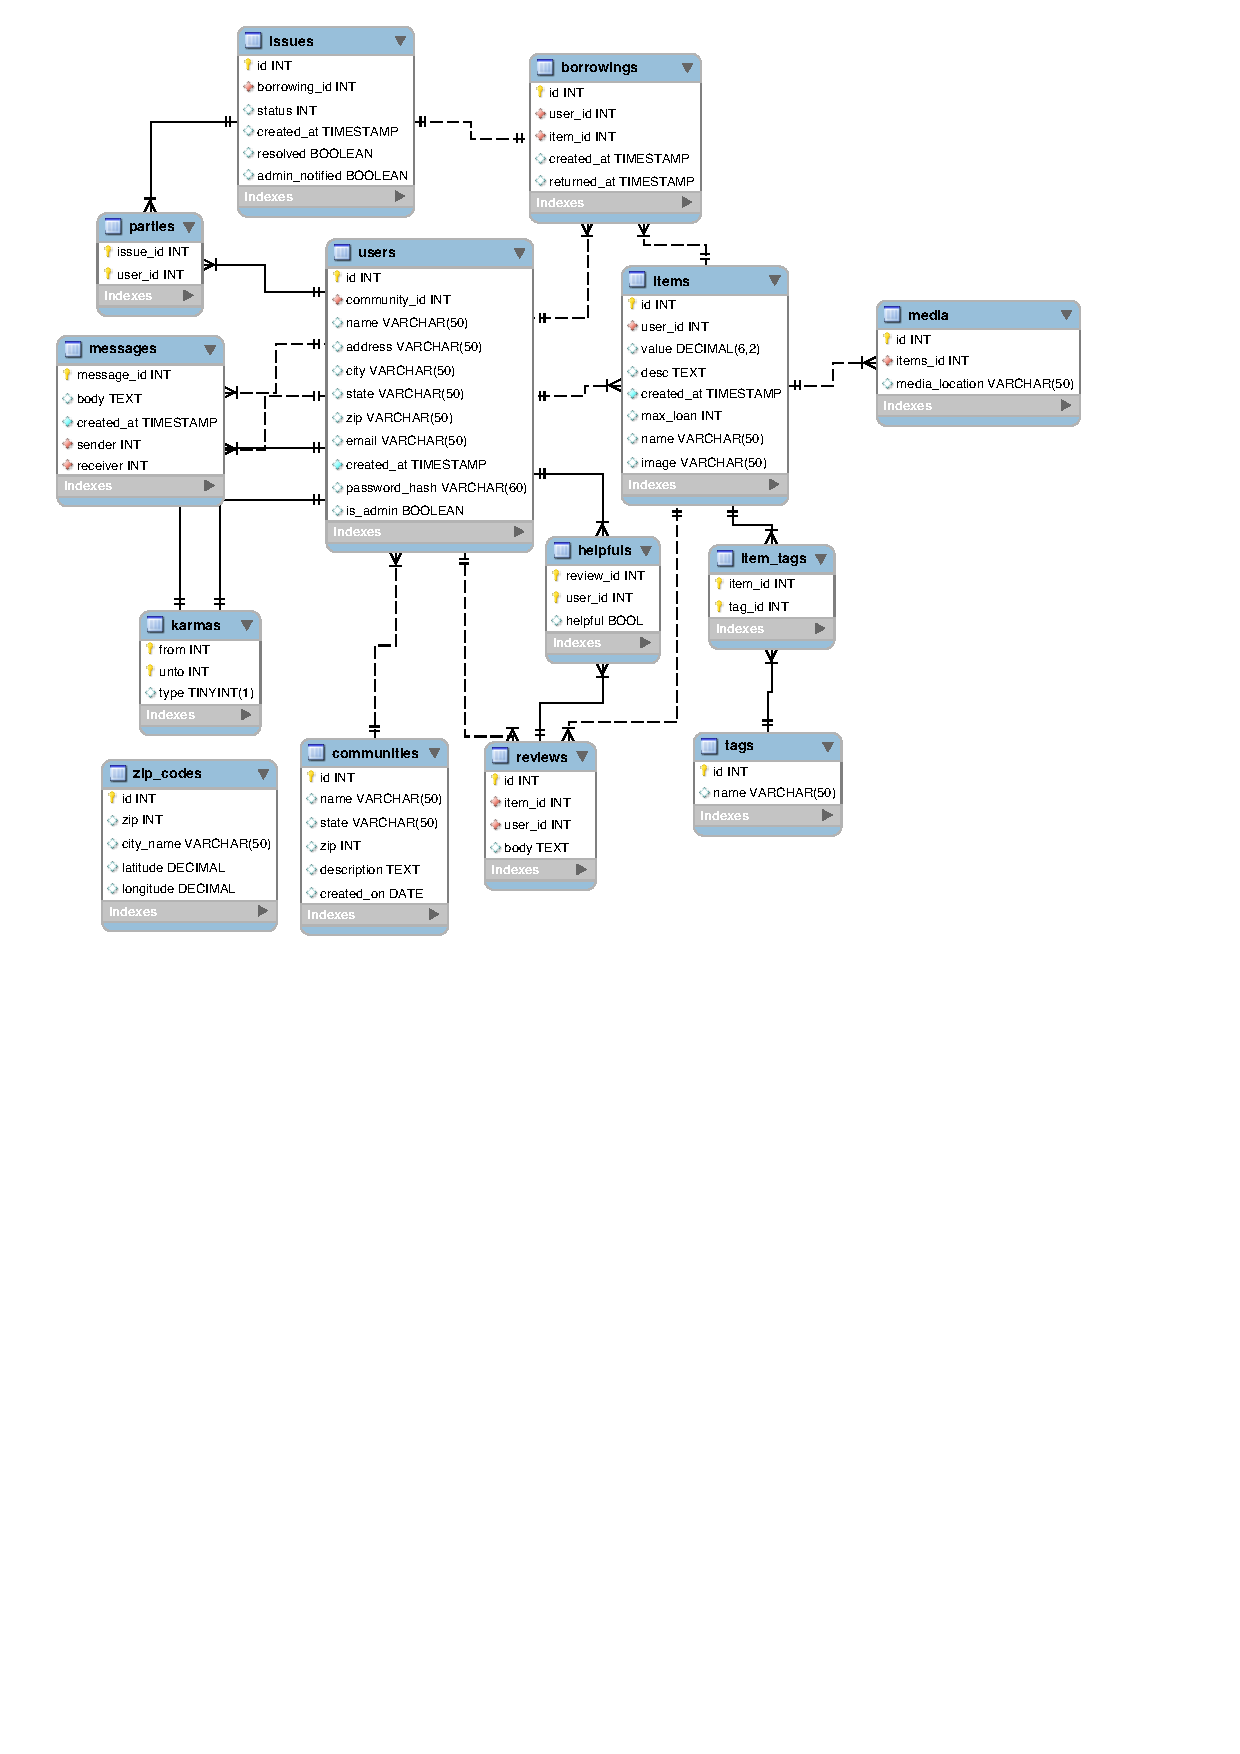
\includegraphics[width=\textwidth]{EECS341Relational.pdf}
    \caption{Relational Diagram for Share*Match}
    \label{fig:RelationalDiagram}
\end{figure*}

\section{Creating Our Database}
% From Project Proposal 3
Our SQL Create Table commands are listed at the end as Figure \ref{fig:SQLCreateCommands}.
\begin{figure*}[p]
    \begin{verbatim}
    CREATE TABLE "borrowings" ("borrow_id" INTEGER NOT NULL PRIMARY KEY 
      AUTOINCREMENT, "borrow_at" TIMESTAMP, "user_id" INTEGER, "item_id" INTEGER);

    CREATE TABLE "helpfuls" ("review_id" INTEGER NOT NULL, "user_id" INTEGER 
      NOT NULL, "helpful" BOOLEAN, PRIMARY KEY("review_id", "user_id"));

    CREATE TABLE "issues" ("issue_id" INTEGER NOT NULL PRIMARY KEY 
      AUTOINCREMENT, "created_at" TIMESTAMP);

    CREATE TABLE "items" ("id" INTEGER NOT NULL PRIMARY KEY AUTOINCREMENT, 
       "value" DECIMAL(6, 2), "created_at" TIMESTAMP, "max_loan" INTEGER, 
       "user_id" INTEGER);

    CREATE TABLE "karmas" ("from" INTEGER NOT NULL, "unto" INTEGER NOT NULL, 
        "type" BOOLEAN, PRIMARY KEY("from", "unto"));

    CREATE TABLE "locations" ("zip_code" INTEGER NOT NULL, "description" TEXT, 
        "created_on" DATE, PRIMARY KEY("zip_code"));

    CREATE TABLE "media" ("media_id" INTEGER NOT NULL PRIMARY KEY AUTOINCREMENT, 
        "item_id" INTEGER, "media_location" VARCHAR(50));

    CREATE TABLE "messages" ("message_id" INTEGER NOT NULL PRIMARY KEY 
        AUTOINCREMENT, "body" TEXT, "created_at" TIMESTAMP, "sender" INTEGER, 
        "reciever" INTEGER);

    CREATE TABLE "parties" ("issue_id" INTEGER NOT NULL, "user_id" INTEGER 
        NOT NULL, PRIMARY KEY("issue_id", "user_id"));

    CREATE TABLE "reviews" ("item_id" INTEGER NOT NULL, "user_id" INTEGER NOT 
        NULL, "body" TEXT, PRIMARY KEY("item_id", "user_id"));

    CREATE TABLE "taggings" ("item_id" INTEGER NOT NULL, "tag_id" INTEGER NOT 
        NULL, PRIMARY KEY("item_id", "tag_id"));

    CREATE TABLE "tags" ("tag_id" INTEGER NOT NULL PRIMARY KEY AUTOINCREMENT, 
        "name" VARCHAR(50));

    CREATE TABLE "users" ("id" INTEGER NOT NULL PRIMARY KEY AUTOINCREMENT, 
        "name" VARCHAR(50), "address" VARCHAR(50), "location_id" INTEGER, 
        "email" VARCHAR(50), "joined_at" TIMESTAMP, "password" INTEGER);
    \end{verbatim}
    \
    caption{SQL CREATE Commands}
    \label{fig:SQLCreateCommands}
\end{figure*}

\section{SQL Queries in RA and TRC}
\section{Integrity Constraints}
\section{Relational Database Design}
\section{Revisiting the Relational Database Schema}
\section{DBMS Implementation}
\section{Application Implementation}
\section{Revisiting the Whole Project}
% This section must be completed by everyone separately.
\section{Team Work}
% This section must be completed by everyone separately.
\section{Conclusions}
\section{Appendix 1: Installation Manual}
\section{Appendix 2: Users Manual}
\section{Appendix 3: Programmer's Manual}

\end{document}
